\chapter{BER理論値を指標とする送信電力制御適用型使用チャネル足切りアルゴリズム
}
本章では,第3章で提案した既存のPPLアルゴリズムについて,研究背景,問題提起をしたのち,これに対する
改善案として3つの内容を検証する.1つ目に伝搬路のSN比が既知であるとしたときのBER理論値を基準とした
獲得固有ベクトル足切りアルゴリズム,2つ目に送信電力分配による理論BER最小化,そして3つ目に,
以上の2つの内容を同時適用した場合を検証する.

\section{研究背景}
第3章では,チャネル推定を行った後に合成チャネル行列を計算して固有値分解する
従来のVCに対して,べき乗法を基本原理とするPPLによる固有ベクトル獲得を提案した.
PPLの最大の特徴は,チャネル推定・合成チャネル行列計算・固有値分解の膨大な演算を,極めて簡単な
非線形処理と無線機間反復処理に置き換えることにある.つまり,伝搬路情報を経由せずに
直接的に固有値・固有ベクトルを求めることができる点に強みがある.
しかし,現在のPPLにおける固有値・固有ベクトルの獲得にかかる無線機間往復数では,実用には十分でないという
問題点がある.固有値問題の性質上,解法には反復解法を用いざるを得ない.PPLではべき乗法を
基本原理としているため,ある程度の反復回数の増加は避けられない.また,VCという方式自体としても
いくつかの課題を有している.その一つに,固有ベクトルに対応する固有値の大きさが,
そのままそのチャネルの利得になっているという特徴上,利得の小さい
チャネルを使用して伝送したデータが,他のチャネルを使用した場合と比較して誤りやすくなるという
問題がある.本章では,上記の二つの問題点に焦点を当て,3つの内容に分けて検証を行う.

\section{検討内容}
ここでは,全部で3つの内容について検討を行う.まず,1つ目としてPPLの課題である無線機間往復数に
対して,一定の通信品質を満たさないチャネルをBER理論値に基づいて足切りすることによる往復数削減
を検証する.2つ目に,VCの課題として挙げた低利得チャネルの誤り率増加減少に対して,送信電力制御
適用によるBER理論値最小化を行う.最後に,1つ目の足切りアルゴリズムに対して,送信電力制御を
組み込んだ場合について検証を行っていく.

\subsection{BER理論値を指標とする使用チャネル足切りアルゴリズム}
ここでは,BER理論値を指標とする使用チャネル足切りアルゴリズムについて解説を行う.
従来のPPLでは,反復処理を行う際,求めたい固有ベクトルの数をあらかじめ
決めたうえで,すべての固有ベクトルが収束するまで反復を行っている.しかし,これは反復回数の面
では無駄が多い.理由として主に以下の3つが挙げられる.1つ目に,べき乗法の特徴として,固有値を大きい順に並べた際に,隣の
固有値との比が大きいほど固有ベクトルの収束が速くなり,逆に小さいほど遅くなるという点が挙げられる.
つまり,求めたい固有ベクトルのうち小さい固有値に対応するものほど,必然的に前の固有値との
比が小さくなるため,獲得までに多くの反復回数を
要することになる.2つ目に,3.5節で説明したように,第2固有ベクトルの獲得では第1固有ベクトルを,
第3固有ベクトルの獲得では第1・第2固有ベクトルを必要とするように,
各固有ベクトルの獲得精度はそれ以前の固有ベクトルの獲得精度の影響を強く受ける.そのため,
後半になるにしたがって,固有ベクトルの獲得精度が低くなり,全体として見たとき拡散符号全体の
直交性が悪化してしまう.3つ目に,固有値が小さい,後半のベクトルほど誤り率が高くなるという
点が挙げられる.VCにおいて,固有値の大きさは各チャネルの利得に対応している.そのため,
固有値の小さいチャネルほど,受信される信号電力が低くなるので,SN比が低下し誤りやすくなるという
特徴がある.上記の理由から,小さい固有値に対応する後半の固有ベクトルを,適切に足切りする
ことができれば,実質的な通信品質を損なわずに不要な反復回数を削減できると考えられる.

図 \ref{figCutoff}に足切りアルゴリズムの概略図,図 \ref{figCutoffFlow}に足切りアルゴリズムのフローチャートを示す.
なお,図 \ref{figCutoff}の固有ベクトル導出に必要な処理は簡略版を示している.
\begin{figure}
    \centering
    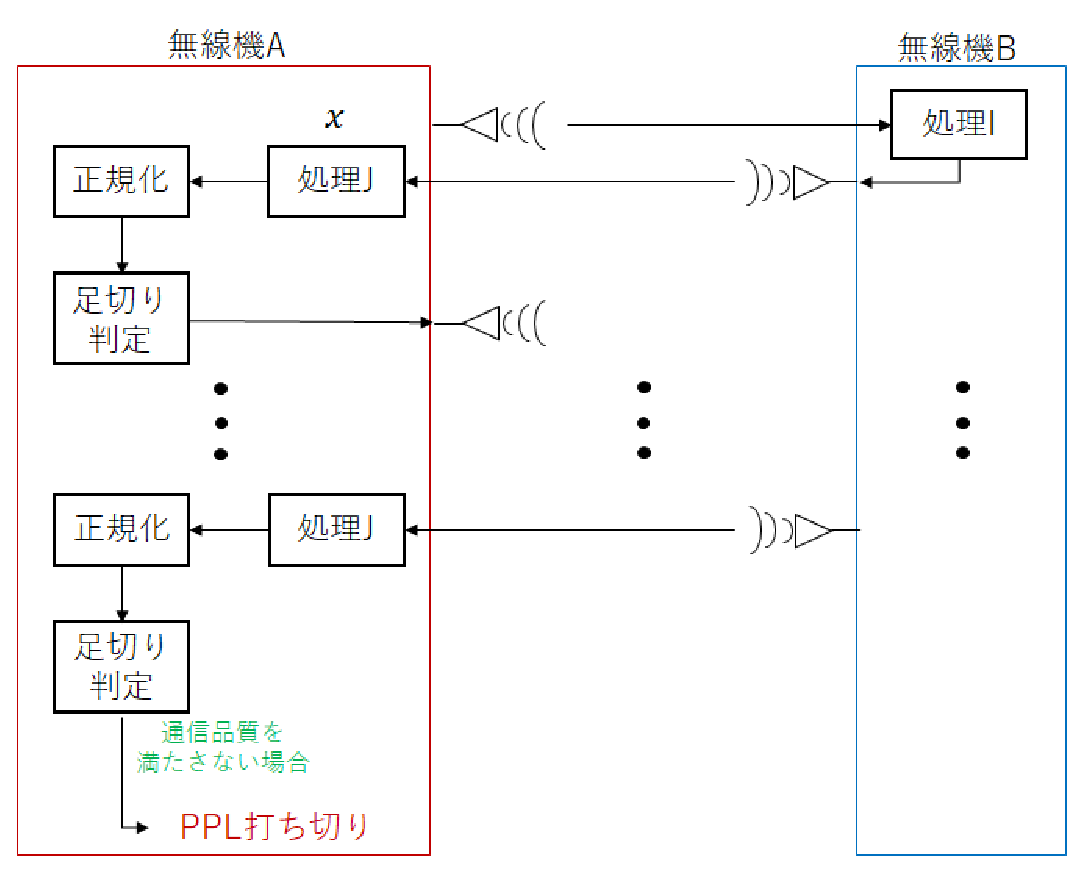
\includegraphics[width=\linewidth]{chapter4/figure/Cutoff.eps}
    \caption{足切りアルゴリズム概略図}
    \label{figCutoff}
\end{figure}
\begin{figure}
    \centering
    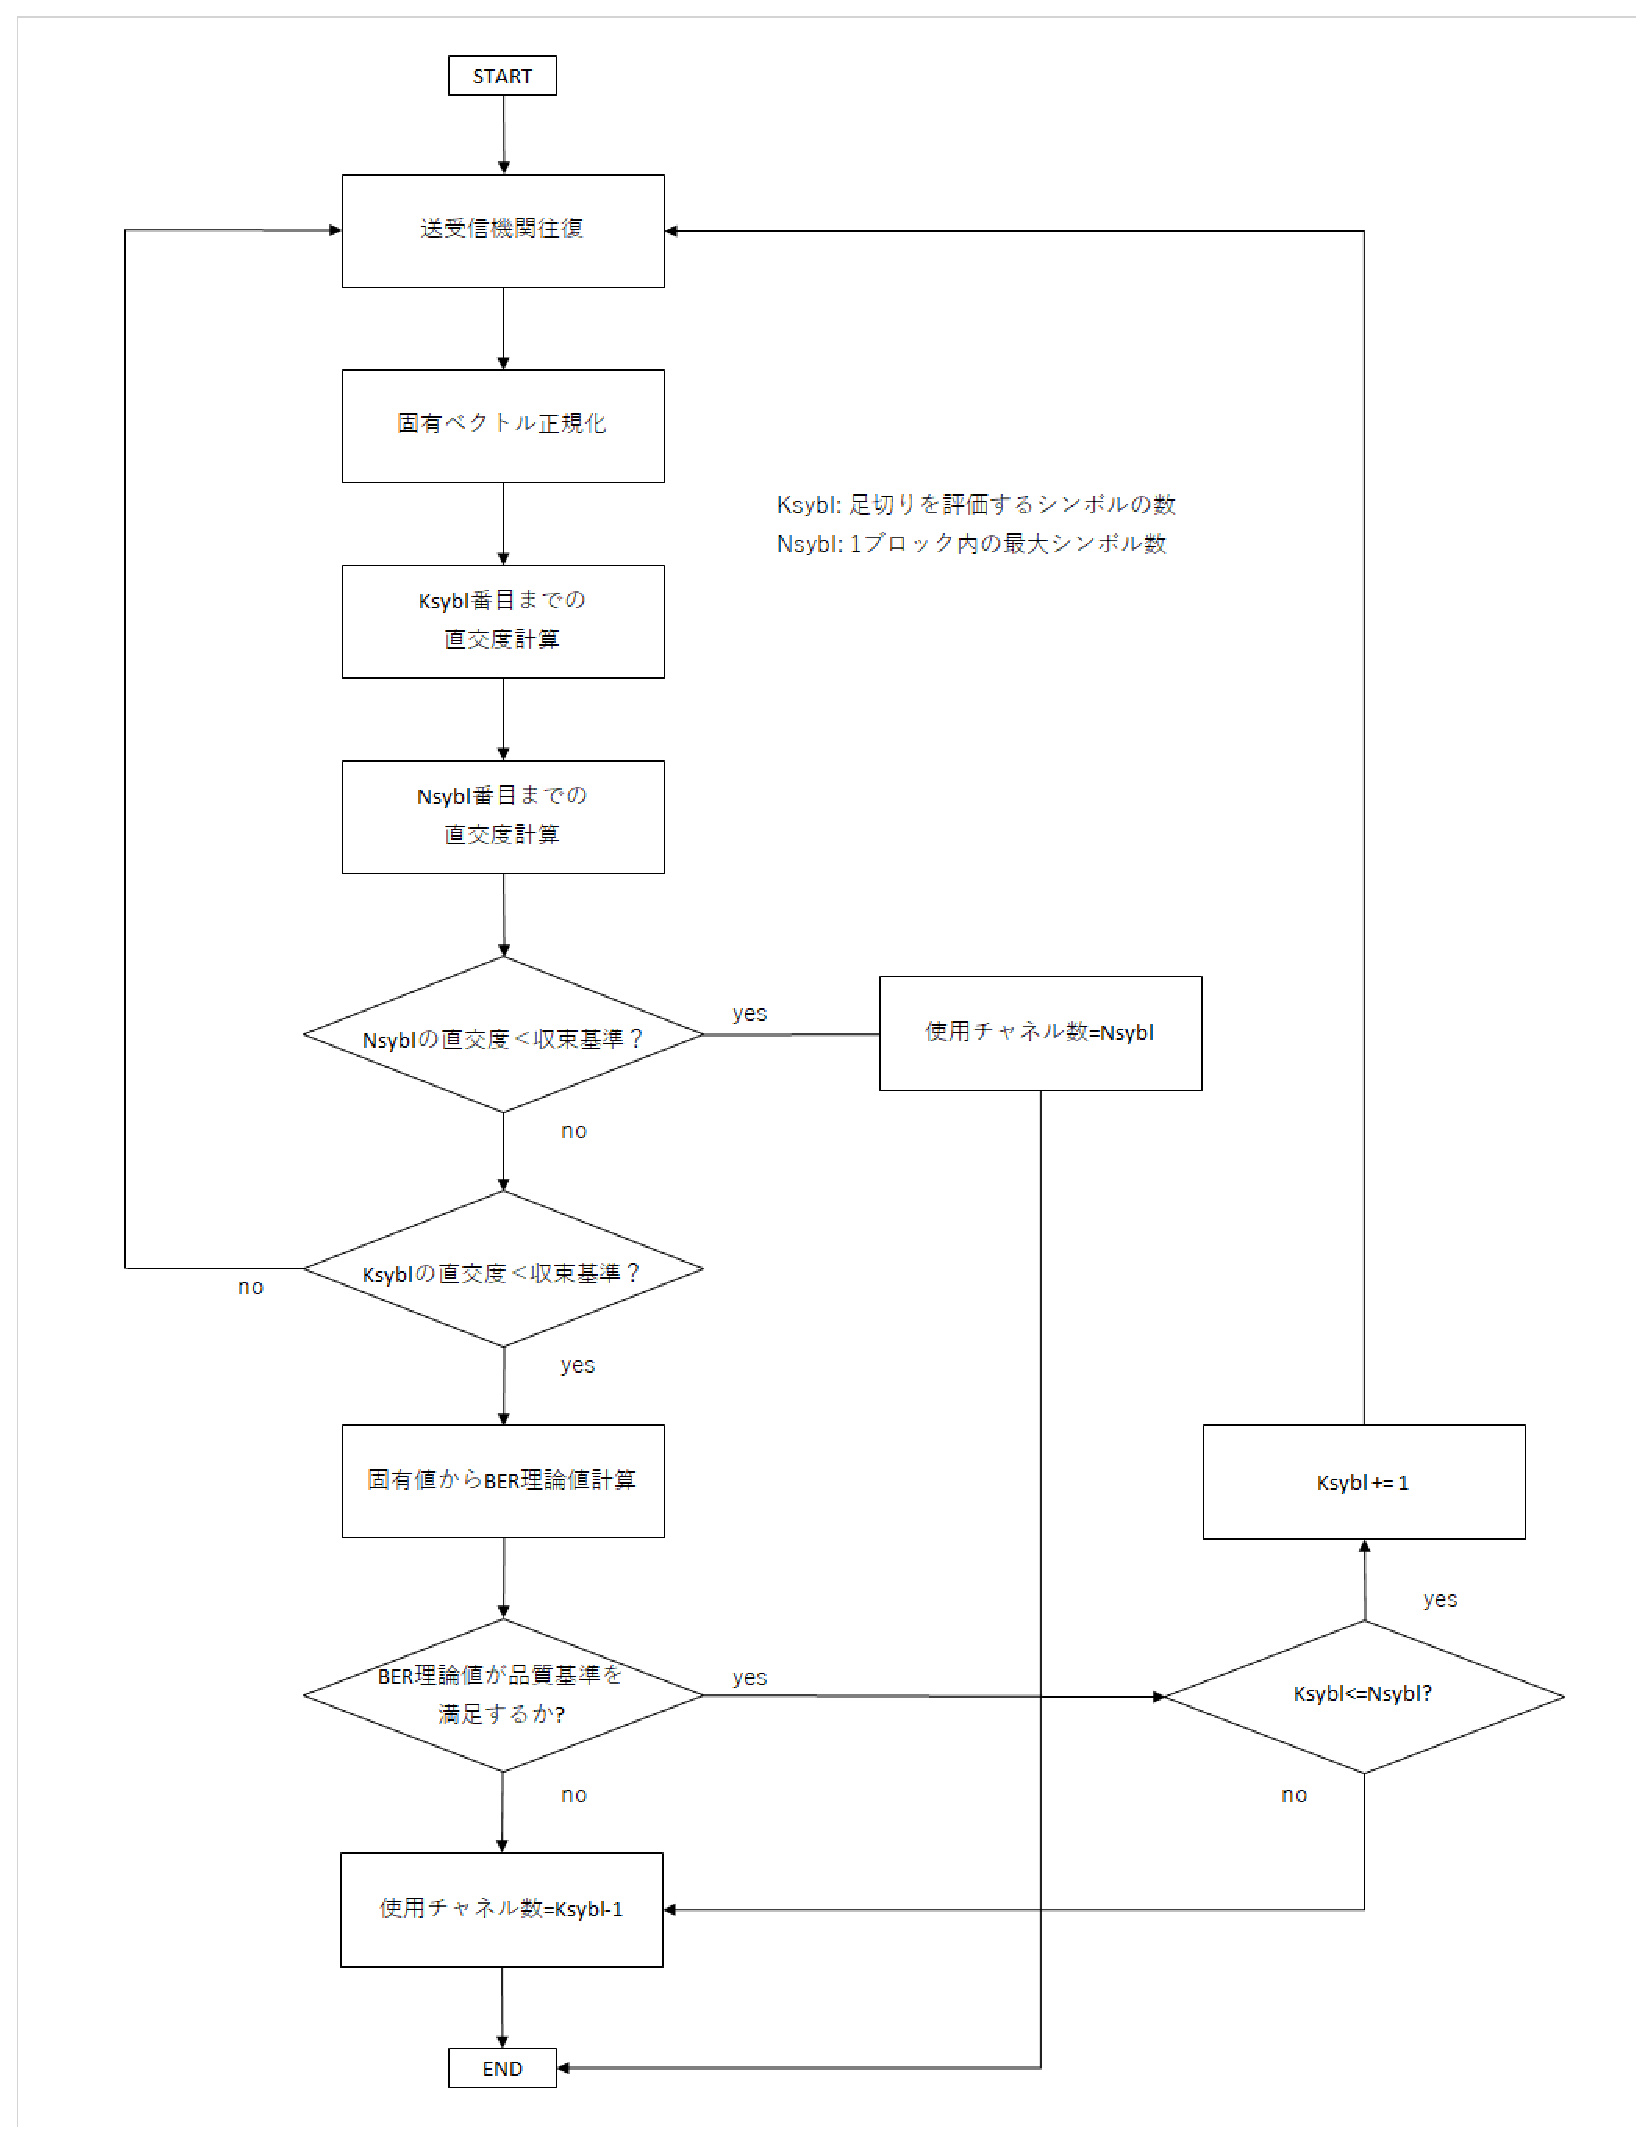
\includegraphics[width=0.95\linewidth]{chapter4/figure/CutoffFlow.eps}
    \caption{足切りアルゴリズムフローチャート}
    \label{figCutoffFlow}
\end{figure}
図 \ref{figCutoffFlow}のNsyblは最大獲得固有ベクトル数,Ksyblは足切り評価を行う固有ベクトル数に
なっている.また,固有ベクトルの収束判定基準に使用する直交度は以下のように定義するものとする.\\
\vspace{5mm}
(例) \quad 固有ベクトルが$\bm{u_1,u_2,u_3}$の3つの場合を考える.
\begin{equation}
    直交度 = \left|\bm{u_1^Hu_2}\right|+\left|\bm{u_1^Hu_3}\right|+\left|\bm{u_2^Hu_3}\right|
\end{equation}

具体的にどのように足切り判定が行われるか図 \ref{figCutoffFlow}をもとに説明する.
当該アルゴリズムは大きく分けて3つの段階に分かれている.
一つ目に無線機間往復,2つ目に獲得固有ベクトルの収束判定,そして3つ目に,収束した固有ベクトルを
用いた場合の通信品質がある基準を満たしているかのBER判定である.
まず,1つ目の無線機間往復について,これは第3章に説明したように非線形処理と正規化を伴う一連の
処理である.次に収束判定についてだが,これはKsybl番目までの固有ベクトルの直交度を求めて,
求めた値が事前に設定した収束基準を満たせば収束したとするものである.収束基準は実験的に求めた
値を使用する.
\begin{equation}
    Ksybl番目までの直交度 \leq 収束基準
\end{equation}
となれば,Ksybl番目までの固有ベクトルが求まったと判断する.
最後に,2つ目の収束判定を合格した固有ベクトルを使用した場合のBER理論値を計算し,
これがあらかじめ設定したBER基準を満たさなければ,Ksybl番目以降の固有ベクトルは獲得する必要がない
として無線機間往復を打ち切る.ここで,Ksybl番目までの固有ベクトルを使用する際の
BER理論値は以下の式,
\begin{equation}
    BER = \frac{1}{Ksybl}\sum_{i=1}^{Ksybl} \frac{1}{2}erfc\left( \sqrt{\lambda_i\frac{E_b}{N_0}} \right)
\end{equation}
で与えられる.上記のBER理論値はQPSKを変調方式として用いた場合のものである.
 \cite{akaiwa}なお,$erfc(x)$は相補誤差関数,$E_bN_0$は伝搬路の1ビット当たりの信号電力
対雑音電力比で,$E_bN_0$は既知とする.このBER理論値が,
\begin{equation}
    BER > BER基準
\end{equation}
を満たす場合,Ksybl番目を含めた通信品質が所望品質を満たさないとして,Ksybl-1番目までを
使用チャネルとしてPPLを打ち切る.ここで,BER基準は$10^{-2}$以下の誤り率であれば,
誤り訂正符号適用時に誤りを復元できるとして,$BER基準=10^{-2}$に設定する.
以上が当該アルゴリズムの解説になるが,1点補足として直交度の
計算部分にKsybl番目までとNsybl番目までの2通りの直交度を計算する部分がある.これは,
アルゴリズムの性質上Ksybl番目までの直交度よりNsybl番目までの直交度の方が早く収束する場合が
稀に存在するため,無線機間往復数が当該アルゴリズムを適用しない場合より増加しないようにするため
挿入している.

\subsection{送信電力制御を用いたBER理論値最小化}
ここでは,送信電力制御によるBER理論値最小化手法について解説を行う.
BER理論値の最小化は,各チャネルに割り当てられる送信電力を変数としたとき,目的関数である
BER理論値を最小とするような送信電力の組み合わせを見つける最適化問題を解くことで得られる.
以下で,式を用いて具体的に説明していく.

まず,変調方式にQPSKを使用する際のBER理論値は(4.3)式と同様に以下で表される.
\begin{equation}
    \frac{1}{N} \sum_{i=1}^N \frac{1}{2}erfc\left( \sqrt{\lambda_i\frac{E_b}{N_0}} \right)
\end{equation}
\begin{equation}
    \left[
        \begin{array}{l}
            N:1ブロック当たりのシンボル数 \\
            \lambda_i:i番目の固有ベクトルに対応する固有値 \\
            E_bN_0:平均E_bN_0
        \end{array}
    \right. \nonumber
\end{equation}
ここに,送信電力$p$を挿入することで,最小化する目的関数,
\begin{equation}
    f(p_1,p_2,\ldots,p_N) = \frac{1}{N} \sum_{i=1}^N \frac{1}{2}erfc\left( \sqrt{p_i\lambda_i\frac{E_b}{N_0}} \right)
\end{equation}
を得る.
また,送信電力$p_i$に関して,全送信電力の合計がNになるということと,各送信電力が非負であるので,
\begin{eqnarray}
    h(p_1,p_2,\ldots,p_N) = \sum_{i=1}^N p_i-N=0 \\
    p_i \geq 0 \hspace{10mm} (i=1,2,\ldots,N)
\end{eqnarray}
の等式制約,不等式制約を考慮する必要がある.(4.7),(4.8)式の制約条件から,この最適化問題はKKT条件と
なっている.以上の最適化問題をラグランジュの未定乗数法を用いて解いていく.
ラグランジュの未定乗数法は2.4.2節で示した通りだが,ここでは問題を簡単にするために一旦
(4.8)式は無視し,等式制約のみの場合で考える.これによって,一般的に解くことが難しいとされる
KKT条件を等式条件のみの最適化問題に帰着させる.さらに,目的関数fが相補誤差関数で表され積分を
含むため,計算が非常に困難になる.そこで,この関数fをチェルノフ限界(Chernoff bound) \cite{akaiwa},
\begin{equation}
    Q(x) = \frac{1}{2}erfc\left( \frac{x}{\sqrt{2}} \right) \leq \exp\left( -\frac{x^2}{2} \right)
\end{equation}
を用いて以下のように近似する.
\begin{equation}
    \frac{1}{N}\sum_{i=1}^N \frac{1}{2}erfc\left( \sqrt{p_i\lambda_i\frac{E_b}{N_0}} \right)
    \leq \frac{1}{N}\sum_{i=1}^N exp \left( -p_i\lambda_i\frac{E_b}{N_0} \right)
\end{equation}
ラグランジュ関数$L$は(2.11)式より,
\begin{equation}
    L(p_1,p_2,\ldots,p_N,\mu) = f(p_1,p_2,\ldots,p_N)-\mu h(p_1,p_2,\ldots,p_N)
\end{equation}
で表され,
\begin{equation}
    \frac{\partial L}{\partial p_i}=\frac{\partial L}{\partial \mu}=0 \hspace{10mm} 
    (i=1,2,\ldots,N)
\end{equation}
を解くことで解が得られる.(4.12)式より,これを(4.6)式,(4.7)式に当てはめると,
\begin{eqnarray}
    \frac{\partial L}{\partial p_i}&=&-\frac{\lambda_i}{N}\frac{E_b}{N_0}
    exp\left( -\lambda_i\frac{E_b}{N_0}p_i \right)-\mu=0 \hspace{10mm} (i=1,2,\ldots,N) \\
    \frac{\partial L}{\partial \mu}&=&p_1+p_2+\cdots+p_N-N=0
\end{eqnarray}
となる.(4.13)式より,
\begin{eqnarray}
    -\frac{\lambda_i}{N}\frac{E_b}{N_0}
    exp\left( -\lambda_i\frac{E_b}{N_0}p_i \right)-\mu &=& 0 \nonumber \\
    exp\left( -\lambda_i\frac{E_b}{N_0}p_i \right) &=& -\frac{N}{\lambda_i\frac{E_b}{N_0}}\mu \nonumber \\
    -\lambda_i\frac{E_b}{N_0}p_i &=& ln\left( -\frac{N}{\lambda_i\frac{E_b}{N_0}}\mu \right) \hspace{10mm} (両辺lnをとる) \nonumber \\
    -\lambda_i\frac{E_b}{N_0}p_i &=& ln\left( -\mu \right) + ln\left( \frac{N}{\lambda_i\frac{E_b}{N_0}} \right) \nonumber \\
    p_i &=& -\frac{1}{\lambda_i\frac{E_b}{N_0}}\left( ln\left( -\mu \right) + 
    ln\left( \frac{N}{\lambda_i\frac{E_b}{N_0}} \right) \right) \hspace{10mm} (i=1,2,\ldots,N)
\end{eqnarray}
となる.(4.15)式を(4.14)式に代入すると,
\begin{eqnarray}
    -\frac{1}{\frac{E_b}{N_0}}\sum_{i=1}^N \frac{1}{\lambda_i}
    \left( ln\left( -\mu \right)+ln\left( \frac{N}{\lambda_i\frac{E_b}{N_0}} \right) \right)-N &=& 0 \nonumber \\
    -\frac{ln(-\mu)}{\frac{E_b}{N_0}}\sum_{i=1}^N \frac{1}{\lambda_i} &=& 
    N+\frac{1}{\frac{E_b}{N_0}}\sum_{i=1}^N \frac{1}{\lambda_i}ln\left( \frac{N}{\lambda_i\frac{E_b}{N_0}} \right) \nonumber \\
    ln(-\mu) &=& -\frac{E_b}{N_0}\frac{1}{\sum_{i=1}^N \frac{1}{\lambda_i}} 
    \left( N+\frac{1}{\frac{E_b}{N_0}}\sum_{i=1}^N \frac{1}{\lambda_i}ln\left( \frac{N}{\lambda_i\frac{E_b}{N_0}} \right) \right)
\end{eqnarray}
と,$ln(-\mu)$が求められる.また,以上より(4.15)式に(4.16)式を代入することで各$p_i$を求めることができる.

ここまでは,(4.8)式の不等式制約を無視して計算を行ったが,実際に(4.15)式を解くと,
\begin{equation}
    p_k < 0 \hspace{10mm} (1 \leq k \leq N)
\end{equation}
のような$p_k$が存在する場合がある.送信電力が負になることはありえないので,
$p_k$のうち最小の$p_k$を$p_{min}$とおいて,
\begin{equation}
    p_i = p_i-(p_{min}-c) \hspace{10mm} (i=1,2,\ldots,N)
\end{equation}
のように全体を正方向に$p_{min}-c$だけシフトさせる.この時$c$は任意の最小送信電力とする.
全体をシフトさせた後,送信電力の合計がNになるように全体を正規化してやれば,各$p_i$の相対的な
大小関係を保ったまま,負となる変数を無くすことができる.つまり,(4.8)式の不等式制約も満足
させることができる.以上が,BER理論値を最小化する送信電力制御の方針である.

\subsection{送信電力制御適用時の使用チャネル足切りアルゴリズム}
ここでは,4.2.1節,4.2.2節で説明した足切りアルゴリズムと送信電力最適化の2つを同時適用した場合に,
送信電力制御によって所望の通信品質を満足するチャネル数を最大化しつつ,不要なチャネルを足切りする
アルゴリズムを提案する.



\section{検証}
\subsection{BER理論値を指標とする使用チャネル足切りアルゴリズム}
\subsubsection{シミュレーション諸元}
\subsubsection{シミュレーション結果}
\subsection{送信電力制御を用いたBER理論値最小化}
\subsubsection{シミュレーション諸元}
\subsubsection{シミュレーション結果}
\subsection{送信電力制御適用時の使用チャネル足切りアルゴリズム}
\subsubsection{シミュレーション諸元}
\subsubsection{シミュレーション結果}
